\section{\acf{SERA}: Features and Limitations}
\label{sub:sera:features_limitations}

Revisiting Section~\ref{sub:sec:SERA}, the \ac{SERA} framework is built on top of \textit{Thalamus} network, where \textit{Thalamus} clients communicate with one another through network messages. For example, \textit{Effector Thalamus} clients, in order to change agent's behaviour have to contact \textit{Skene} that processes and redirects the request to the most suitable clients: \textit{Nutty Tracks} for animations and \textit{Speech Server} for utterances. In addition, it has a finer control over the agent's action, able to, for example, causing delays or generate idle behaviour.

\ac{SERA} already assures a decoupled design for agents by using different \textit{Thalamus} clients with different responsibilities, cooperating with one another through well-defined \textit{Thalamus} network messages. Moreover, there is already support for interrupting ongoing actions, however, we need to assess how well \textit{SERA} agents are capable to quickly adapt to the dyadic state of the interaction. To this end, we ran the tests described in the following paragraphs.

In the first test, we measured the response speed between requesting an action and its execution. Following Figure~\ref{fig:solution:sera_simple_message_delay}, an \textit{Effector} \textit{Thalamus} client (in the role of a potential rapport strategy) sends an utterance request to the \textit{Skene} client. The request is dispatched and processed in \textit{Skene} and redirected to the \textit{Speech Server} which executes the desired utterance. However, each network message has to pass through \textit{Thalamus} so that it can redirect the messages to the target clients in the network. The test was successful although:

\begin{itemize}
	\item If a speech request arrives while there is one in execution, the \textit{Speech Server} executes them sequentially which can have undesired effects. For example, an \textit{Effector} may request utterance twice as a reaction to the external environment making the \textit{Speech Server} run them both twice, one after another, regardless of their duration;
	\item There is a noticeable (less than a second) delay between the requests and the effects, as requests pass firstly through \textit{Skene}, \textit{Thalamus} and finally, either \textit{Nutty Tracks} or \textit{Speech Server} (Figure~\ref{fig:solution:sera_simple_message_delay} and~\ref{fig:solution:sera_complex_message_delay}).
\end{itemize}

\begin{figure}[H]
	\centering
	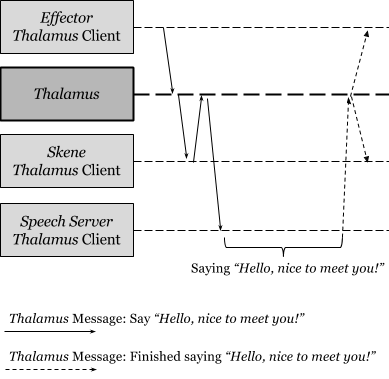
\includegraphics[width=0.45\textwidth]{images/SERA_SimpleTest.png}	
	\caption{\textit{Thalamus} network messages sent when attempting to execute a vocalisation.}
	\label{fig:solution:sera_simple_message_delay}
\end{figure}

In the second test, we extended the first test to examine the behaviour when interrupting actions (Figure~\ref{fig:solution:sera_complex_message_delay}). The sender requests an utterance to be executed, then interrupts it while it is still in execution. This test was not successful as there was a substantial delay between requesting the interruption and the effect ($\approx$ 3 seconds average in 10 tests).

\subsection*{Discussion}

We repeated the tests described in the previous section with animations instead of utterances but the results were identical. We strongly believe that the results are affected by the network nature of \ac{SERA}. When sending the messages directly from the \textit{Skene}'s \ac{GUI}, the delays were substantial shorter, reduced to less than a second, compared to the previous 3 seconds when sending from a separate client to \textit{Skene} as described in Figure~\ref{fig:solution:sera_simple_message_delay} and Figure~\ref{fig:solution:sera_complex_message_delay}.

To sum up, to accomplish our goals, taking into account \textit{Skene}'s capabilities and the tests previously described, the framework needs to:
\begin{itemize}
	\item Reduce the number of network messages that pass through the network, in order to reduce the latency between the requests and the effects, without breaking compatibility with current agents;
	\item Distribute \textit{Skene} responsibilities to different independent components in order to promote modularisation, and give the researchers the ability to customise the agent's behaviour more easily.
\end{itemize}


\begin{figure}[H]
	\centering
	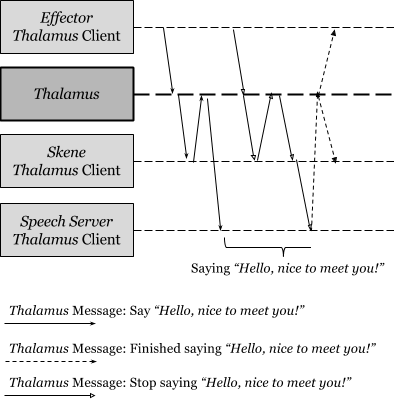
\includegraphics[width=0.45\textwidth]{images/SERA_DelayTest.png}
	\caption{\textit{Thalamus} network messages sent when attempting to execute and interrupt a vocalisation.}
	\label{fig:solution:sera_complex_message_delay}
\end{figure}
